\documentclass[Main]{subfiles}
\begin{document}

\chapter{Indledning}

\section{Formål}


\subsection{Regler og valg af Frekvens}
Der er mange regler inden for trådløs kommunikation, så hvilke frekvenser er lovlige at udnytte uden licens?

Det er de fleste i ISM-båndet, da de er lavet til  Industriel, videnskabelig og medicinsk bånd. Grunden til det ikke er alle er at der er lokale krav, alt efter hvor man er i verden. Eks har USA meget komplekse krav til 433MHZ.\cite[s. 32]{Lov1}

De meste gængse frekvenser der er kan benyttes i industrien og til hobby brug er derfor:

\begin{itemize}
\item 433 MHz
\item 868 MHz
\item 915 MHz
\item 2.4 GHz
\item 5.8 GHz
\end{itemize}

Så der skal vælges en frekvens af disse.
Den frekvens der egner sig bedst dette projekt, er den frekvens der rækker længst. 

\begin{figure}[H]
\centering
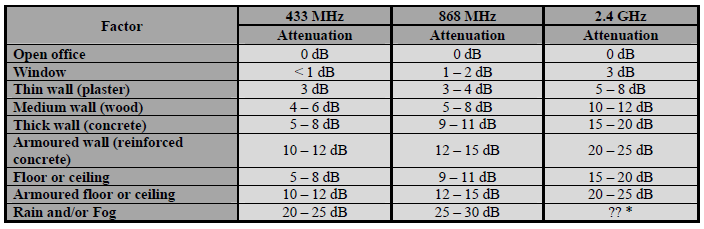
\includegraphics[scale=1]{FrekvensDempning}
\caption{Frekvens dæmpning - Figuren viser tests udfør af Telit wireless solutions et stort italiensk firma med speciale i trådløs teknologi.}
\end{figure}




Som man det ses på figures over så er der mindre modstand i objekter, desto længere man kommer ned i frekvens.
I og med at næsten alle hobby entusiaster inden for RC fly, bruger 2.4 GHz. 
Bliver valget for dette projekt 433 MHz.

\subsection{Valg af sender}

Når det var valgt at projektet skulle benytte 433MHz. Skulle der findes en sender/modtager.
Valget faldt på en chip fra Texas Instruments cc1101, Grundet dens mange muligheder.
Nogle af de ting som projektet kunne drage fordel af var;

\begin{itemize}
\item Flere kanaler
\item Variable datahastighed (0.6 to 600 kbps)
\item Gode pakkehåndterings muligheder 
\item Flere frekvenser, hvor 433MHz er en af dem
\item Programmerbar power output
\item Spi interface
\end{itemize}

Denne chip var også nemt tilgængelig på diverse online sider som ebay. Hvilket betyder at den chip bliver brugt i vid udstrækning og dermed er prisen fornuftig.
\\
\subsection{Valg af Microcontroller til fjernbetjening}

Det var allerede forudbestemt at denne skulle benytte en atmel AVR chip, da der var kendskab til denne type chips.

Det der skulle bestemmes var hvilken Chip i atmels serie.

\begin{itemize}
\item Spi
\item I2C
\item external interrupts pins
\end{itemize}

Det viste sig at de mindste chips som levede op til disse krav er;

\begin{itemize}
\item ATtiny88
\item atmega8
\item atmega16
\item atmega32
\end{itemize}


Disse chips opfyldte kravene til chippen der skulle bruges.
Så der skulle ses på andre faktorer, for at vælge en. 
Det blev pris, der afgjorde dette.\\\\
ATtiny88 - 46,91 kr.\\
Atmega8  - 7,71 kr.\\
Atmega16 - 21,40 kr.\\
Atmega32 - 36,29 kr.\\
\\(prisen - I skrivende stund, på ebay, for dip versionen, inc. porto)
\\Derfor blev valget en atmega8.
\subsection{Regler og valg af Frekvens}
Der er mange regler inden for trådløs kommunikation, så hvilke frekvenser er lovlige at udnytte uden licens?

Det er de fleste i ISM-båndet, da de er lavet til  Industriel, videnskabelig og medicinsk bånd. Grunden til det ikke er alle er at der er lokale krav, alt efter hvor man er i verden. Eks har USA meget komplekse krav til 433MHZ.\cite[s. 32]{Lov1}

De meste gængse frekvenser der er kan benyttes i industrien og til hobby brug er derfor:

\begin{itemize}
\item 433 MHz
\item 868 MHz
\item 915 MHz
\item 2.4 GHz
\item 5.8 GHz
\end{itemize}

Så der skal vælges en frekvens af disse.
Den frekvens der egner sig bedst dette projekt, er den frekvens der rækker længst. 

\begin{figure}[H]
\centering
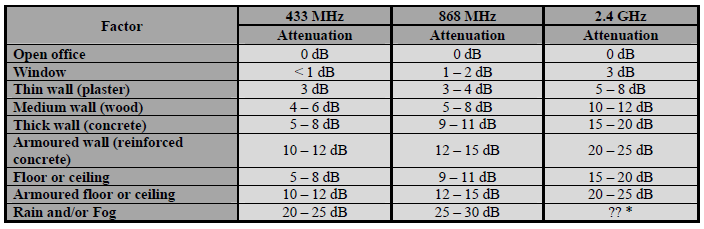
\includegraphics[scale=1]{FrekvensDempning}
\caption{Frekvens dæmpning - Figuren viser tests udfør af Telit wireless solutions et stort italiensk firma med speciale i trådløs teknologi.}
\end{figure}




Som man det ses på figures over så er der mindre modstand i objekter, desto længere man kommer ned i frekvens.
I og med at næsten alle hobby entusiaster inden for RC fly, bruger 2.4 GHz. 
Bliver valget for dette projekt 433 MHz.

\subsection{Valg af sender}

Når det var valgt at projektet skulle benytte 433MHz. Skulle der findes en sender/modtager.
Valget faldt på en chip fra Texas Instruments cc1101, Grundet dens mange muligheder.
Nogle af de ting som projektet kunne drage fordel af var;

\begin{itemize}
\item Flere kanaler
\item Variable datahastighed (0.6 to 600 kbps)
\item Gode pakkehåndterings muligheder 
\item Flere frekvenser, hvor 433MHz er en af dem
\item Programmerbar power output
\item Spi interface
\end{itemize}

Denne chip var også nemt tilgængelig på diverse online sider som ebay. Hvilket betyder at den chip bliver brugt i vid udstrækning og dermed er prisen fornuftig.
\\
\subsection{Valg af Microcontroller til fjernbetjening}

Det var allerede forudbestemt at denne skulle benytte en atmel AVR chip, da der var kendskab til denne type chips.

Det der skulle bestemmes var hvilken Chip i atmels serie.

\begin{itemize}
\item Spi
\item I2C
\item external interrupts pins
\end{itemize}

Det viste sig at de mindste chips som levede op til disse krav er;

\begin{itemize}
\item ATtiny88	\cite{AtmelTiny}
\item atmega8	\cite{AtmelMega8}
\item atmega16	\cite{AtmelMega16}
\item atmega32  \cite{AtmelMega32}
\end{itemize}


Disse chips opfyldte kravene til chippen der skulle bruges.
Så der skulle ses på andre faktorer, for at vælge en. 
Det blev pris, der afgjorde dette.\\\\
ATtiny88 - 46,91 kr.\\
Atmega8  - 7,71 kr.\\
Atmega16 - 21,40 kr.\\
Atmega32 - 36,29 kr.\\
\\(prisen - I skrivende stund, på ebay, for dip versionen, inc. porto)
\\Derfor blev valget en atmega8.


\end{document}
